\documentclass{scrartcl}
\usepackage{polski}
\usepackage[utf8]{inputenc}

\usepackage{hhline}
\usepackage{enumerate}
\usepackage{graphicx}
\usepackage{epstopdf}
\usepackage{float}
\usepackage{amsmath}
\usepackage{geometry} 
\usepackage{multirow}
\usepackage{mathtools}
\usepackage{paralist}
\usepackage{listings}
\usepackage{xpatch}


\newgeometry{tmargin=2.5cm, bmargin=2.5cm, lmargin=2.4cm, rmargin=2.4cm} 

\title{Metody planowania i analizy eksperymentów\\Zadanie domowe 1}
\subtitle{Analiza zbioru danych \textit{Abalone}}

\author{\textbf{Prowadzący:} dr inż. Adam Zagdański \\ 
        \textbf{Student:} Piotr Bielak, 218 137\\WT TN 9:15}

\date{Wrocław, 14 kwietnia 2018r.}

\begin{document}
\maketitle

\section{Wprowadzenie}
Do realizacji zadania domowego użyto zbiór danych \textbf{Abalone}, który został
zaczerpnięty z repozytorium danych \textit{UCI Machine Learning Repository}. 
Zbiór ten zawiera dane opisujące ślimaki morskie i został przygotowany w celu 
predykcji ich wieku. Wśród atrybutów można wyróżnić jedną cechę jakościową oraz 
8 cech ilościowych. Dokładniejsze informacje na ich temat zostały przedstawione
w Tabeli 1. W celu przeprowadzenia analizy został wykorzystany język R w oparciu
o wbudowane pakiety tego języka (brak dodatkowych zewnętrznych pakietów).

\section{Analiza}
  Jedyną cechą jakościową w tym zbiorze danych jest \textit{płeć}. Dostępne są 
  tutaj 3 wartości: żeńska, męska i nieokreślona, która występuje w przypadku
  młodych osobników. Dla pozostałych cech zostały wyznaczone wartości minimalne,
  maksymalne oraz średnia i odchylenie standardowe (jako, że to są cechy mierzalne).

  \begin{table}[H]
    \center
    \begin{tabular}{|c|c|c|c|c|c|}
      \hline
      \textbf{Nazwa atrybutu} & \textbf{Komentarz}      & \textbf{Min} & \textbf{Max} & \textbf{Średnia} & \textbf{Odchyl. stand.} \\ \hline
      \textit{Sex}            & płeć; cecha jakościowa  & \multicolumn{4}{|c|}{żeńska, męska, nieokreślona} \\ \hline \hline
      \textit{Length}         & długość pancerza (mm)   & 0.075        & 0.815        & 0.524            & 0.120 \\ \hline
      \textit{Diameter}       & średnica (mm)           & 0.055        & 0.650        & 0.408            & 0.099 \\ \hline
      \textit{Height}         & wysokość (mm)           & 0.000        & 1.130        & 0.140            & 0.042 \\ \hline
      \textit{Whole weight}   & całkowita waga (g)      & 0.002        & 2.826        & 0.829            & 0.490 \\ \hline
      \textit{Shucked weight} & waga mięsa (g)          & 0.001        & 1.488        & 0.359            & 0.222 \\ \hline
      \textit{Viscera weight} & waga wnętrzności po wykrawieniu (g) & 0.001  & 0.760  & 0.181            & 0.110 \\ \hline
      \textit{Shell weight}   & waga pancerza po wysuszeniu (g)     & 0.002  & 1.005  & 0.239            & 0.139 \\ \hline \hline
      \textit{Rings}          & liczba pierścieni; wiek & 1            & 29           & 9.934            & 3.224 \\ \hline
    \end{tabular}
    \caption{Podstawowe parametry atrybutów zbioru Abalone.}
  \end{table}

  Można zauważyć, że wartości atrybutów są bardzo małe -- długości na poziomie 
  prawie jednego milimetra oraz wagi o maksymalnej wartości prawie 3 gramów.
  Odstającym tutaj atrybutem jest liczba pierścieni. Przyjmuje ona dyskretne,
  całkowitoliczbowe wartości z przedziału 1 do 29 (z wyłączeniem 28). Jest ona
  o tyle ważna, że po dodaniu 1.5, otrzymujemy wiek danego ślimaka. Stąd też
  liczba pierścieni oraz wiek będą stosowane zamiennie.

  \pagebreak

  Pierwszym aspektem jaki można przeanalizować jest liczba instancji w zbiorze
  danych względem danej płci. Zależność ta została przedstawiona na Rysunku 1.
  Jak widać, dla każdej płci zostało zebranych porównywalnie wiele przykładów (ok. 1300),
  przy czym osobników o płci męskiej zbadano o 15\% więcej (ok. 1500 egzemplarzy).

  \begin{figure}[H]
    \center
    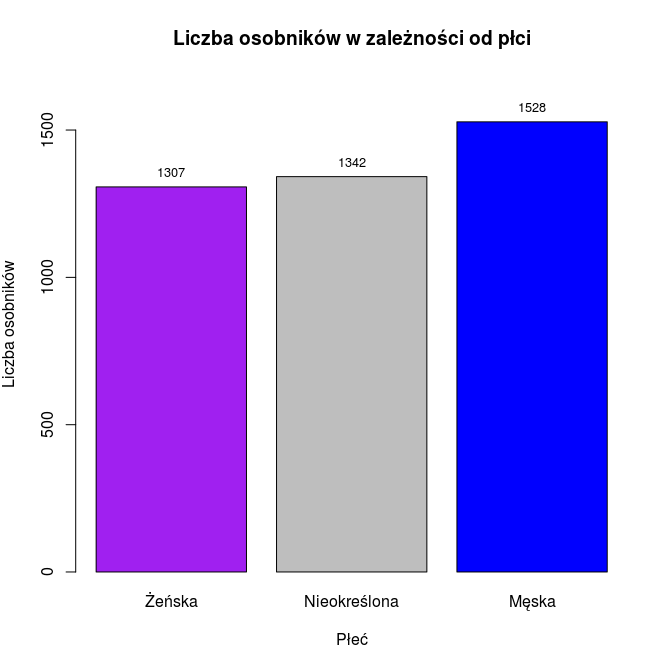
\includegraphics[width=0.6\textwidth]{plots/barplot_nb_instances.png}
    \caption{Wykres zależności liczby osobników w zależności od płci.}
  \end{figure}

  Kolejnym krokiem jest wizualizacja rozkładów wartości atrybutów ilościowych.
  Dla każdego atrybutu zostały przedstawione:
  \begin{itemize}
    \item{histogram; z szerokością przedziału obliczaną z reguły \textit{Freedmana-Diaconisa},}
    \item{średnia próbkowa,}
    \item{mediana próbkowa,}
    \item{rozkład normalny parametryzowany wartościami atrybutu,}
    \item{funkcja przybliżająca histogram (estymator jądrowy).}
  \end{itemize}

  Rysunek 2 przedstawia powyższe elementy dla całego zbioru danych.
  Można tutaj zauważyć, że zarówno długość (Length) oraz średnica (Diameter)
  mają bardzo poodbne rozkłady wartości, przesunięte o około 0.1 względem
  wartości średniej. Oba rozkłady są ponadto lewostronnie skośne. Również
  dla atrybutów związanych z wagą (Whole weight, Shucked weight, Viscera weight
  oraz Shell weight) wykresy wykazują podobieństwo pod względem kształt, są przesunięte
  względem wartości średniej oraz prawostronnie skośne. Jest to związane z silną korelacją
  wartości atrybutów, co zostało przedstawione na Rysunku 3. 

  Szczególnymi przypadkami na Rysunku 2 są wysokość ślimaków (Height) 
  oraz liczba pierścieni (Rings). W przypadku pierwszego można zaobserować,
  że większość wartości jest skupiona w przedziale od 0 do około 0.25, ale
  występują też pojedyncze większe wartości. Skutkuje to w skupieniu / koncentracji
  widocznej części słupków histogramu w poprzednio wspomnianym przedziale. Rozkład
  wartości liczby pierścieni natomiast najbardziej spośród wszystkich, przypomina
  rozkład normalny. Zakładając, że wartości tego atrybutu byłyby zgodne z rozkładem
  normalnym, można by wysunąć wniosek, że najwięcej (99,7 \%) wartości mieści się
  w przedziale 1-19 lat; przedział ten można by wtedy wyznaczyć z reguły 3 sigma, 
  pamiętając, że średnia wieku to około 10 lat, a odchylenie standardowe wynosi 
  około 3 lat. Porównując ten wynik z danymi odczytanymi z wykresu, można zauważyć,
  że są one dość zbliżone.

  \begin{figure}[H]
    \center
    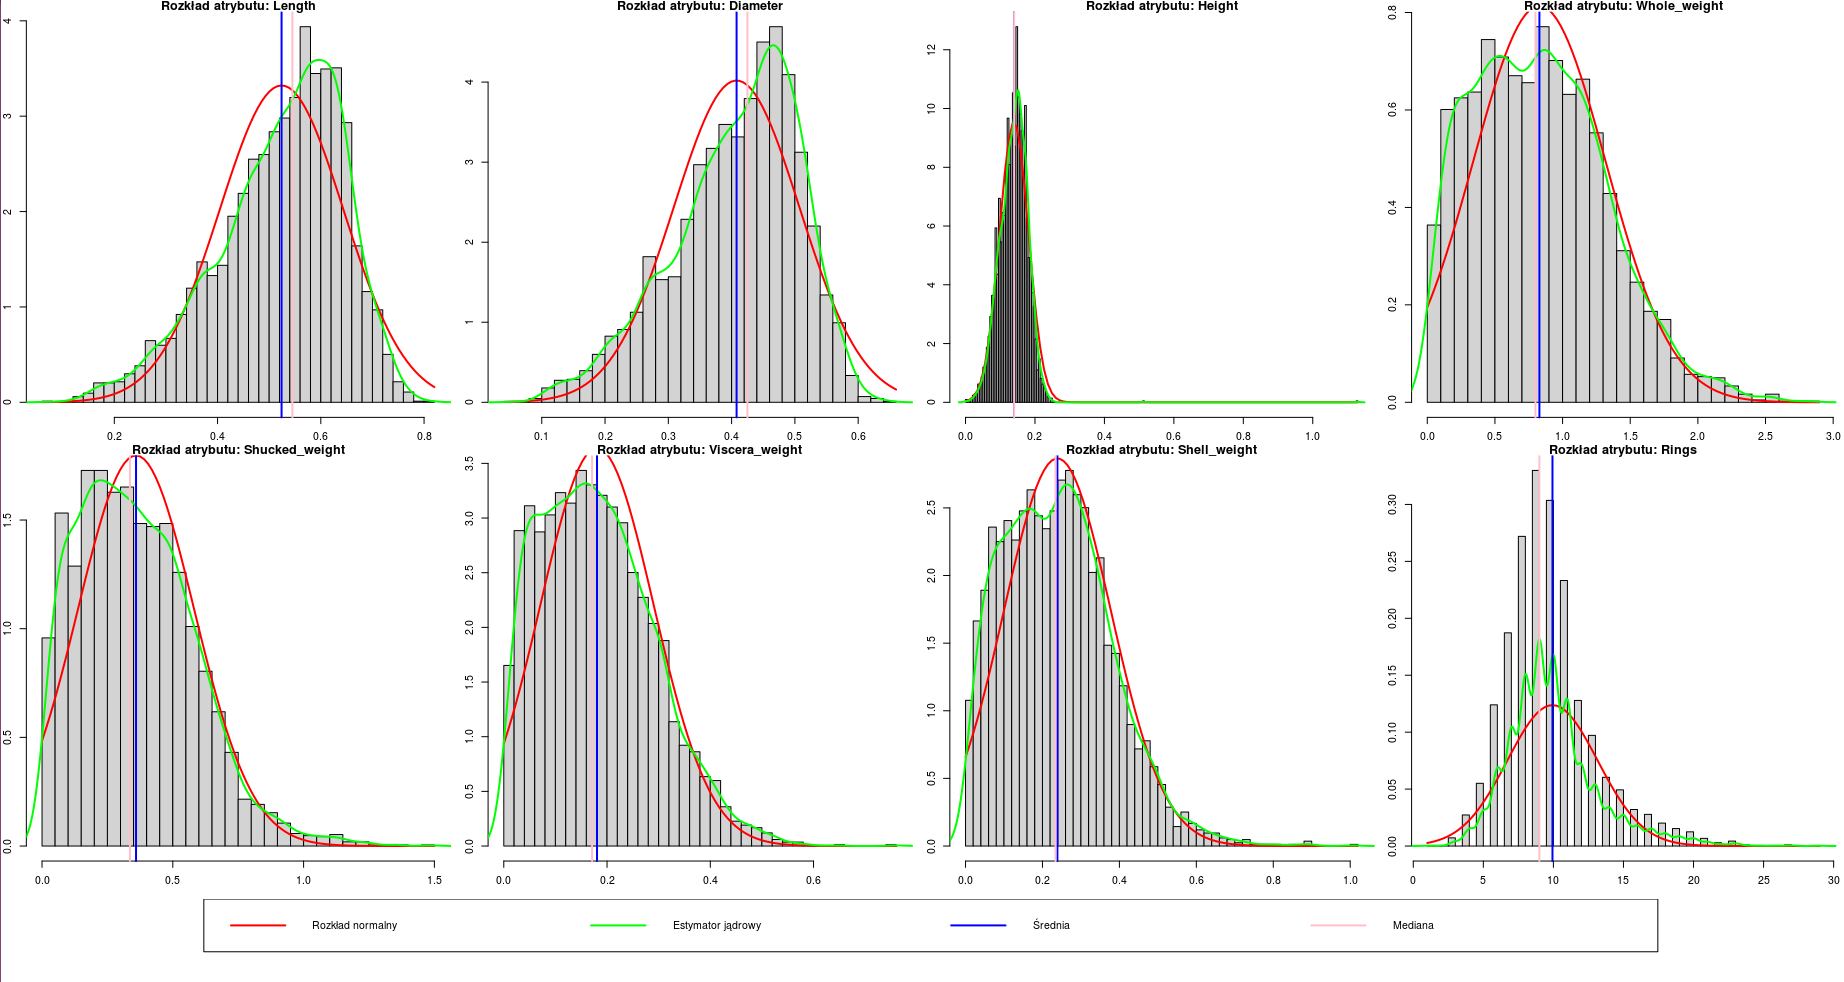
\includegraphics[width=\textwidth]{plots/histograms_full.png}
    \caption{Rozkłady wartości atrybutów (dla całego zbioru).}
  \end{figure}

  \begin{figure}[H]
    \center
    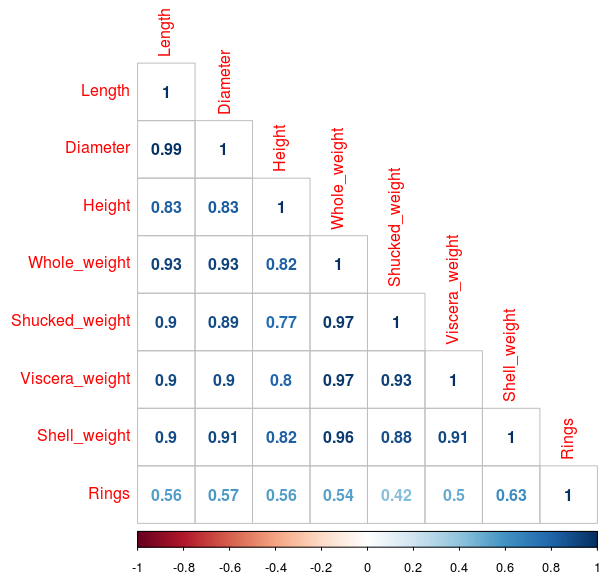
\includegraphics[width=0.6\textwidth]{plots/correlations.png}
    \caption{Korelacja wartości atrybutów w zbiorze danych.}
  \end{figure}

  \pagebreak
  Analizując dokładniej wartości atrybutu liczby pierścieni, ale uwzględniając
  tym razem również płeć osobników otrzymano Rysunek 4. Można zauważyć, że w
  wieku do 8 lat włącznie dominuje płeć nieokreślona (młode osobniki). Pojawiają
  się również osobniki, które już wtedy wykształciły płeć i ich liczba narasta wraz
  z wiekiem. Powyżej 8 lat dominują już osobniki z określoną płcią. Zgodnie z
  obserwacją związaną z analizą Rysunku 1, widać że w zbiorze danych występuje więcej
  instancji, gdzie badany były osobniki męskie -- wyższe niebieskie słupki niż fioletowe
  dla prawie każdej wartości wieku. Od wieku 16 lat poziom liczby osobników męskich 
  i żeńskich się wyrównuje, czasami nawet więcej osobników żeńskich zostało zbadanych.

  \begin{figure}[H]
    \center
    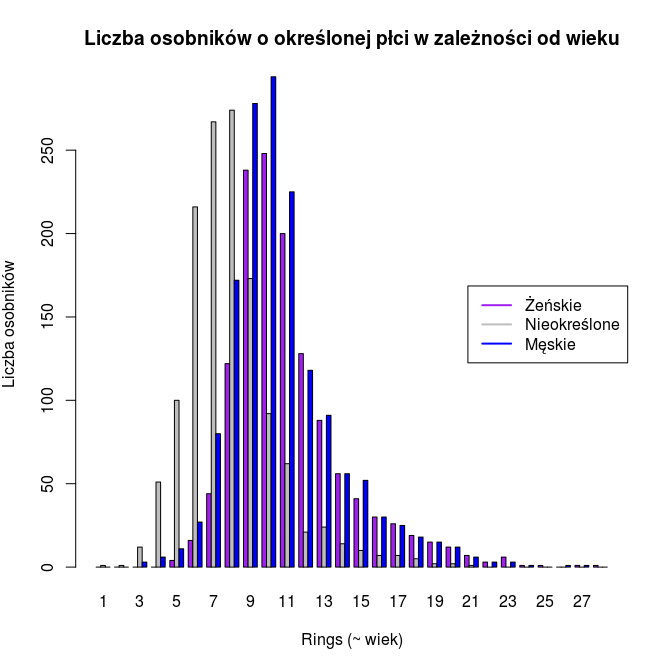
\includegraphics[width=0.8\textwidth]{plots/barplot_age_sex.png}
    \caption{Wykres liczby osobników o określonej płci w zależności od wieku (Rings).}
  \end{figure}

  \pagebreak
  Wykresy pudełkowe (box-plot) potwierdzają wszystkie powyższe obserwacje, tzn.:
  \begin{itemize}
    \item{atrybuty Length oraz Diameter są co do charakteru rozkładu / rozrzutu wartości
          bardzo podobne (jedynie przesunięte co do wartości średniej / mediany); dodatkowo
          na poniższych wykresach można zauważyć, że dla tych atrybutów pojawiają się wartości
          odstające (outlier) tylko w dolnym zakresie wartości,}

    \item{podobnie zachowują się również atrybuty związane z wagą; podobne wysokości
      pudełek oraz wartości odstające tylko dla górnego zakresu wartości,}

    \item{dzięki zastosowaniu wykresów pudełkowych, można również zauważyć wspomnianą wcześniej
      koncentrację wartości atrybutu Height -- pudełko jest bardzo wąskie i posiada kilka wartości
      odstających w górnym zakresie wartości oraz trochę więcej z dolnym zakresie.}
  \end{itemize}
  \begin{figure}[H]
    \center
    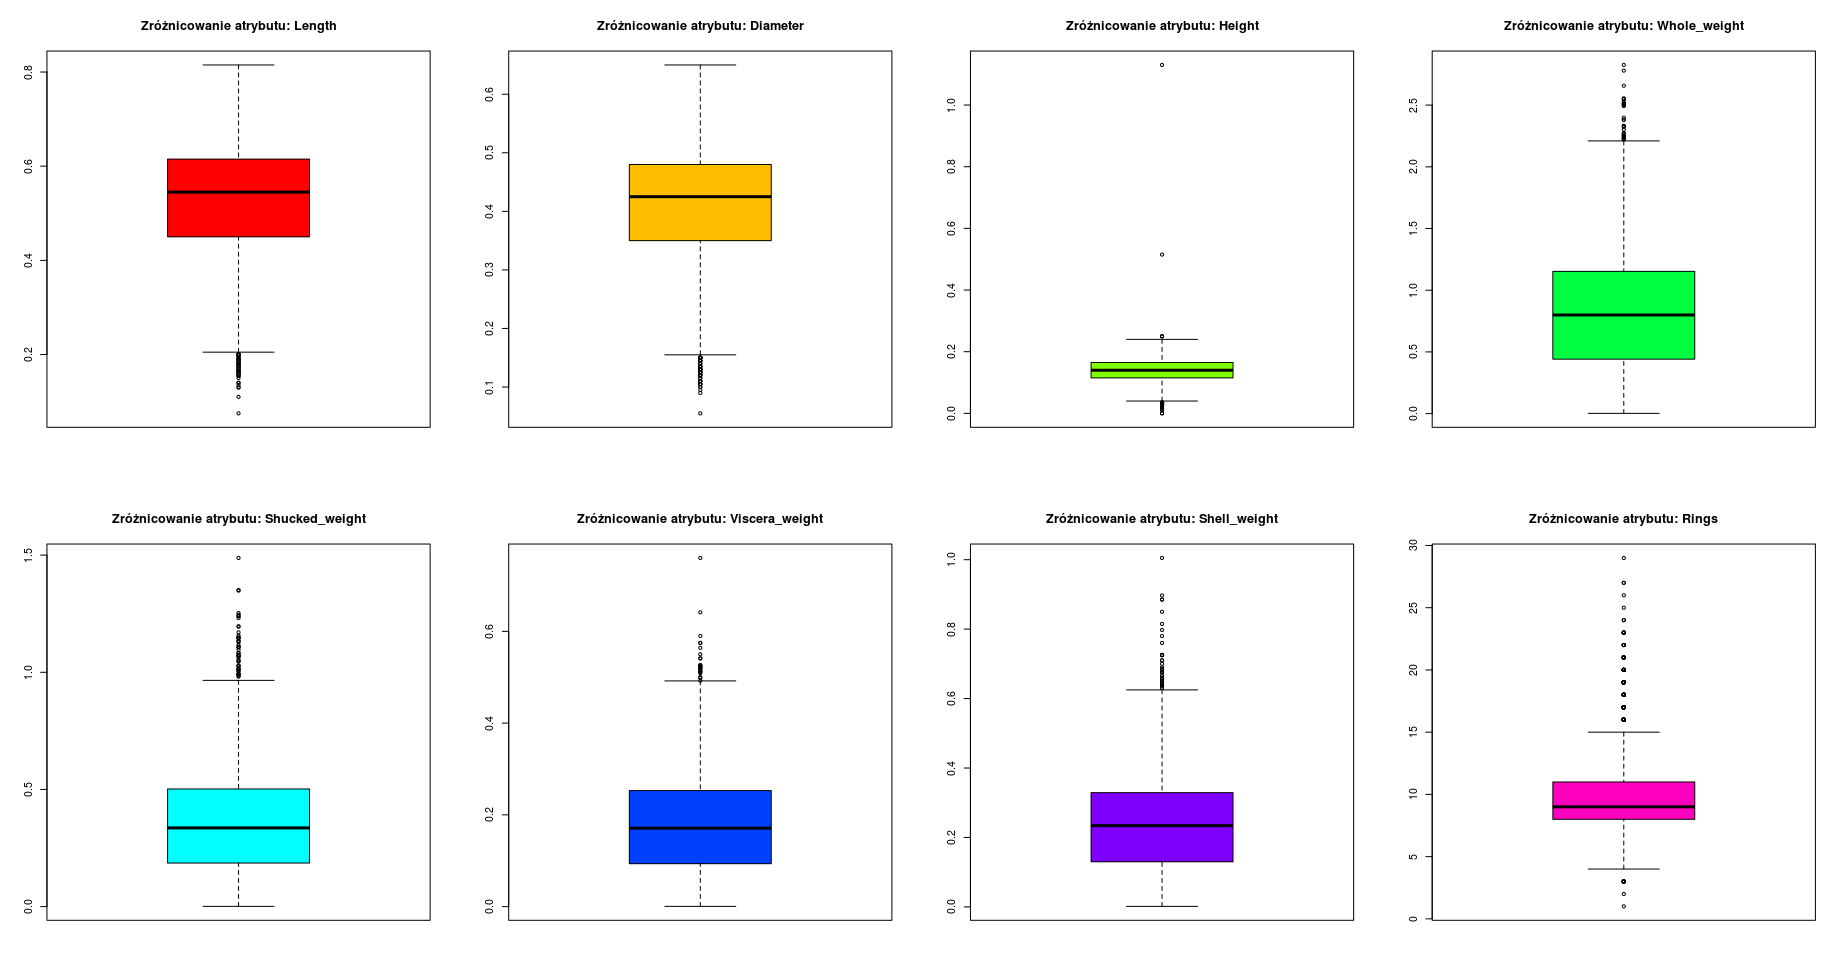
\includegraphics[width=\textwidth]{plots/boxplots.png}
    \caption{Zróżnicowanie wartości atrybutów.}
  \end{figure}
\end{document}


